\documentclass[12pt,letterpaper]{article}

% just for the example
\usepackage{lipsum}
% Set margins to 1.5in
\usepackage[margin=1.5in]{geometry}

% for graphics
\usepackage{graphicx}

% for crimson text
\usepackage{crimson}
\usepackage[T1]{fontenc}
\usepackage{url}

% setup parameter indentation
\setlength{\parindent}{0pt}
\setlength{\parskip}{6pt}

% for 1.15 spacing between text
\renewcommand{\baselinestretch}{1.15}

% For defining spacing between headers
\usepackage{titlesec}
% Level 1
\titleformat{\section}
  {\normalfont\fontsize{18}{0}\bfseries}{\thesection}{1em}{}
% Level 2
\titleformat{\subsection}
  {\normalfont\fontsize{14}{0}\bfseries}{\thesection}{1em}{}
% Level 3
\titleformat{\subsubsection}
  {\normalfont\fontsize{12}{0}\bfseries}{\thesection}{1em}{}
% Level 4
\titleformat{\paragraph}
  {\normalfont\fontsize{12}{0}\bfseries\itshape}{\theparagraph}{1em}{}
% Level 5
\titleformat{\subparagraph}
  {\normalfont\fontsize{12}{0}\itshape}{\theparagraph}{1em}{}
% Level 6
\makeatletter
\newcounter{subsubparagraph}[subparagraph]
\renewcommand\thesubsubparagraph{%
  \thesubparagraph.\@arabic\c@subsubparagraph}
\newcommand\subsubparagraph{%
  \@startsection{subsubparagraph}    % counter
    {6}                              % level
    {\parindent}                     % indent
    {12pt}                           % beforeskip
    {6pt}                            % afterskip
    {\normalfont\fontsize{12}{0}}}
\newcommand\l@subsubparagraph{\@dottedtocline{6}{10em}{5em}}
\newcommand{\subsubparagraphmark}[1]{}
\makeatother
\titlespacing*{\section}{0pt}{12pt}{6pt}
\titlespacing*{\subsection}{0pt}{12pt}{6pt}
\titlespacing*{\subsubsection}{0pt}{12pt}{6pt}
\titlespacing*{\paragraph}{0pt}{12pt}{6pt}
\titlespacing*{\subparagraph}{0pt}{12pt}{6pt}
\titlespacing*{\subsubparagraph}{0pt}{12pt}{6pt}

% Set caption to correct size and location
\usepackage[tableposition=top, figureposition=bottom, font=footnotesize, labelfont=bf]{caption}

% set page number location
\usepackage{fancyhdr}
\fancyhf{} % clear all header and footers
\renewcommand{\headrulewidth}{0pt} % remove the header rule
\rhead{\thepage}
\pagestyle{fancy}

% Overwrite Title
\makeatletter
\renewcommand{\maketitle}{\bgroup
   \begin{center}
   \textbf{{\fontsize{18pt}{20}\selectfont \@title}}\\
   \vspace{10pt}
   {\fontsize{12pt}{0}\selectfont \@author}
   \\ \today

   \end{center}
\egroup}
\makeatother

% Used for Tables and Figures
\usepackage{float}

% For using lists
\usepackage{enumitem}

% For full citations inline
\usepackage{bibentry}
\nobibliography*

% Custom Quote
\newenvironment{myquote}[1]%
  {\list{}{\leftmargin=#1\rightmargin=#1}\item[]}%
  {\endlist}

% Create Abstract
\renewenvironment{abstract}
{\vspace*{-.5in}\fontsize{12pt}{12}\begin{myquote}{.5in}
\noindent \par{\bfseries \abstractname.}}
{\medskip\noindent
\end{myquote}
}

% Set Title, Author, and email
\title{Patents and Litigation in the Video Game Industry}
\author{Ryan Gallagher,
\\ Jam Wilder,
\\ Austin Snyder,
\\ Sean Gallaway}
\date{\today}

\begin{document}
\date{\today}
\maketitle
\thispagestyle{fancy}

\pagebreak

\section{Abstract}
The video game industry is no stranger to wild legal battles. Just as there are patent battles and controversies in any other industry, there are many in the video game industry. What makes these special is that in so many cases, the legal process flies in the face of what the everyday consumer wants. In this paper, we explore three famous legal battles in which the masses can't enjoy widely popular games and mechanics. These cases being:
\begin{itemize}
    \item Nintendo vs PocketPair (The Palworld Lawsuit).
    \item Warner Bros filing a patent over the widely popular Nemesis System.
    \item PUBG vs Epic Games.
\end{itemize}
\par All of these cases have wide implications. PUBG suing Epic Games, those are two of the most popular video games currently, with Fortnite (Epic Games product which caused the lawsuit) being the most popular game in the world. PUBG is essentially suing because the gameplay is strikingly similar. The Nintendo lawsuit is also interesting, in this case, they are suing a similar game, Palworld, on the basis that they hold a patent for throwing a ball to catch creatures in a digital environment. The games are similar no doubt, but with such a broad patent will be interesting to see how the case develops. Perhaps the most infuriating patent case is that of Warner Bros with their Nemesis system. The Nemesis system involved defeating enemies, who then learn the player's patterns and behaviors, and adapt to that for subsequent encounters. It was widely beloved, but now sits idly by until the year 2036 while it is under patent.
\par Common to all of these situations, the consumer is being deprived of a fun experience by the patent laws which are in place. There is an interesting argument to be had about fair use, and taking inspiration from popular works to make a new product which incorporates functionalities which people loved in prior games.

\pagebreak

\section{Introduction}
Throughout the years with the advancements in technology specifically in the niche area of video game creation, the animation style of the games and characters have drawn inspiration from one another and different anime design artist.
This has caused for the probing and enforcement of litigation to protect the intellectual rights to the created property, this has been an ongoing issue for a while in the genre especially when companies refuse to listen to their consumer based groups,
for the features and add-ons to said game, thus forms the creation of a game similar to theirs with the wanted features that the consumers had wanted or the creation of a whole new sub-genre from the main genre of games.


\section {Warner Bros}
In 2016 Warner Bros filed a patent for their "Nemesis System" which saw use in their 'Middle-Earth: Shadow of Mordor' and 'Middle-Earth: Shadow of War' games. This system allows for procedurally created non-player characters to remember previous interactions and react to them.

For example, if a Nemesis was previously defeated with fire, they could come back later with either increased defenses against fire, or a fear of fire. The Nemesis could also change in appearance or behavior due to actions by the player character. Additionally, the faction that these Nemesis characters belong to could change based on player actions as well. If a Nemesis is a captain of a group of soldiers and they get beaten too often, the Nemesis would be demoted, and vice-versa if the Nemesis wins against the player.
\begin{figure}
    \centering
    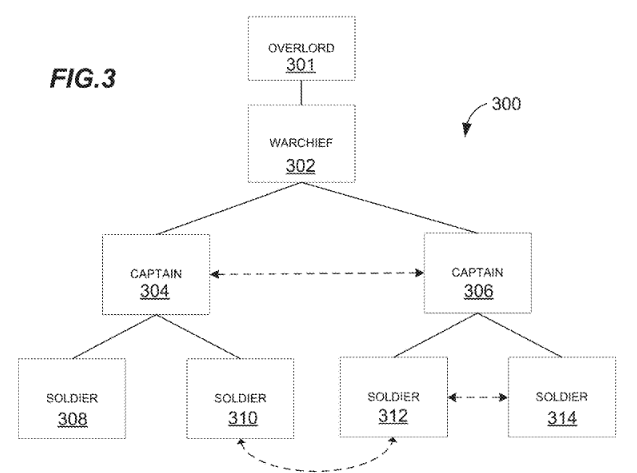
\includegraphics[width=0.5\linewidth]{nemesis.PNG}
    \caption{Heirarchy example shown in \cite{wb}}
    \label{fig:seanpic}
\end{figure}

The patent \cite{wb} filed by Warner Bros specifically targets the section on a Nemesis's rank in a hierarchy, and sending these Nemesis non-player characters over a network to another player under certain circumstances. The vague wording of the patent makes it really difficult for independent developers to know what parts of the Nemesis system is actually under patent.
This confusion has given a lot of developers pause on whether or not they will be litigated against for including similar systems, which gives Warner Bros an edge. The patent was granted in 2021 after being applied for in 2016, and expires in 2036. Warner Bros has not used the Nemesis system since 2017's 'Middle-Earth: Shadow of War', so in addition to the discontent on having a patent on parts of this system, the system its self is not being used.

\section{Wider Issues in the Software World}
These examples are simply ones in which consumers are being deprived of fun experiences in the video game industry. There are many other cases of very similar issues around the wider software world, not just in entertainment, but also products which consumers interact with in their everyday life. Or, even worse, a software company taking advantage of their consumers. There have been many examples thoughout the history of the software industry of this. In fact, it is quite a common issue right now with large language models, since the companies developing them need so much data. They are being accused of copywrite infringement, and theft of intellectual property by many. Worse than this, we may see more cases where companies are outright harming their consumers, as we will discuss with Sony BMG.

\subsection{Soverain Software}
Soverain Software is commonly known as a "patent troll", maintaining many patents not for the purposes of business use, but rather just to claim royalties from others. An everyday example, Soverain Software at one time held a patent for the "digital shopping cart". A digital shopping cart is a feature which is available on most e-commerce websites today, but that may have been impossible without the case we are going to discuss. Soverain Software sued and settled with Amazon, and Gap inc. in 2010, In the U.S. District Court for the Eastern District of Texas. Gap settled without disclosing the terms, but Amazon settled for \$40 million \cite{Soverain}.

After a few more years of suing various other companies for infringing on their digital shopping cart patent, Soverain Software finally was defeated in 2013 in the U.S Court of Appeals for the Federal Circuit. Where several of their judgements were reversed, as being "plain in the view of the prior art", or in other words, people had done similar things before, so it wasn't new or inventive \cite{Soverain}. The U.S. Supreme Court denied Soverain Software's petition to hear their case, and as such the ruling from the Federal Court against Soverain Software stood. Their patents were invalidated, and their lawsuits were killed \cite{Soverain}.

This is a case where the consumer gets a better product, and the software industry prevails. One company doesn't get to hold a patent over a very common practice, and users get to use a simple feature universally across many websites.

\subsection{Sony BMG Copy Protection Scandal}
In 2005, information came out that Sonyn BMG had been installing one of two pieces of software on consumer's machines, unbeknownst to the consumers. This software was actually bunlded directly onto CD's themselves, so a user had no way of expecting this to happen \cite{sony}. These softwares provided digital rights management, they would modify the user's operating system to interfere with copying CD's \cite{sony}. Neither of these two programs could easily be removed from the user's machine as well.

A large issue with this, these two programs that Sony was installing on people's machines were introducing security vulnerabilities, taking system resources, and even causing crashes. Not only were they changing your machine without any sort of permission, they were also installing a program which jeopardized your security. Sony BMG eventually released an uninstaller to get these programs off of a user's machine. In fact, this uninstaller simply made the files invisible, and didn't uninstall anything \cite{sony}. Of course, it also installed additional software which could not be removed easily, and brought on even more security issues \cite{sony}.

Sony BMG eventually ended up paying out several class action lawsuits on the matter. This is a great example of a software company pushing the envelope as far as what they can get away with doing to their consumers. What is quite shocking is how Sony BMG doubled down, and lied to the masses again, simply making files invisible, and then creating even \textbf{more} issues on user machines.

\pagebreak

\begin{thebibliography}{99}

\bibitem{Palworld}
Julia Alexander. \textit{Palworld removes feature following Nintendo lawsuit speculation}. The Verge, 2024.\\
\url{https://www.theverge.com/news/663210/palworld-updates-feature-removed-nintendo-lawsuit}

\bibitem{Nemesis}
Engadget Staff. \textit{Shadow of Mordor’s innovative Nemesis system is locked behind a patent until 2036}. Engadget, 2021.\\
\url{https://www.engadget.com/gaming/shadow-of-mordors-innovative-nemesis-system-is-locked-behind-a-patent-until-2036-195437208.html}

\bibitem{PUBGvsFortnite}
Red Points. \textit{PUBG sues Fortnite: A copyright battle royale}. Red Points Blog, 2022.\\
\url{https://www.redpoints.com/blog/pubg-sues-fortnite-a-copyright-battle-royale/}

\bibitem{Soverain}
Wikipedia. \textit{Soverain Software}. Wikipedia, 2024.\\
\url{https://en.wikipedia.org/wiki/Soverain_Software?utm_source=chatgpt.com}

\bibitem{sony}
Wikipedia. \textit{Sony BMG copy protection rootkit scandal}. Wikipedia, 2024.\\
\url{https://en.wikipedia.org/wiki/Sony_BMG_copy_protection_rootkit_scandal?utm_source=chatgpt.com}

\bibitem{wb}
Michael de Plater et al. \textit{Nemesis characters, Nemesis forts, social vendettas and followers in computer games}. US Patent 10,926,179 B2, 2021.\\
\url{https://patentimages.storage.googleapis.com/45/aa/b5/7d07e883c25b26/US10926179.pdf}

\end{thebibliography}
\end{document}
